\subsection{Iteration 1: JPA data model}
For the initial iteration submission, we have provided an implemented domain using the
Spring JPA framework. The following items were considered in this iteration. The code base will continue to evolve over subsequent iterations.
\begin{itemize}
    \item Version allows for optimistic locking during database transactional contexts to ensure that a stale persistence does not occur.

    \item Created at and updated at values use Spring auditing to add the appropriate system time to our entities upon submission.

    \item Enumerations were provided as separate classes to promote reusability and extensibility within the code base.

    \item Care was given in assigning relationship owning entities to allow for succinct operations in persistence and modification.

    \item At this time, no cascading operation have been determined. This is to be provided later as realization of these operations will become more available while development continues.

    \item Special consideration was given to the Notification entity to ensure that it may have one and only one relationship with the following differing entity types: Post, Event, Media.

    \item Custom user implementation of UserDetails and UserDetailsService (from Spring security) was used to create the base user class. This was chosen since it will provide roles tied to logged in users and can be fetched to determine which options are available to a logged in user based on the granted authorities for that role.
\end{itemize}

\subsection{Iteration 2: REST API implementation of selected use cases}
For the second iteration submission, progress on the source code has been made, including but not limited to:
\begin{itemize}
    \item The creation of controller and service skeletons
    \item The implementation of Use Cases 1 (view media library), 5 (edit event), 7 (view event), 10 (create post), 11 (edit post), 12 (delete post) and 13 (view post).
    \item Preliminary JUnit tests for use cases
\end{itemize}

\subsection{Iteration 3: REST API implementation of all use cases}
For the third iteration submission, REST API implementation of all 12 required use cases has been completed. This includes:
\begin{itemize}
    \item All source code necessary to run endpoints for the 3 assigned use cases per team member plus two additional use cases completed beyond this limit, for a total of 14 use cases of the initial 16 drafted
    \item Full JUnit test suite encompassing all 14 use cases
    \item Postman collection with 24 requests for ease of API use
\end{itemize}

\subsubsection{GitHub Repository}

The source code with JPA \& API implementation is provided in a zip folder along with this document. The latest release is \href{https://github.com/tkm3d1a/cs5324_s24_class_project/releases/tag/0.2}{linked here} on the project GitHub repository. Please refer to the \texttt{README} file in the root directory of the source code zip for deployment instructions and endpoint prerequisites. \\
\\
Issue tracking for Iterations 2 and 3 was completed entirely with GitHub Issues. Below are screenshots of our completed GitHub Issues, our remaining open GitHub Issues, and our completed Pull Requests.

\begin{figure}[H]
    \centering
    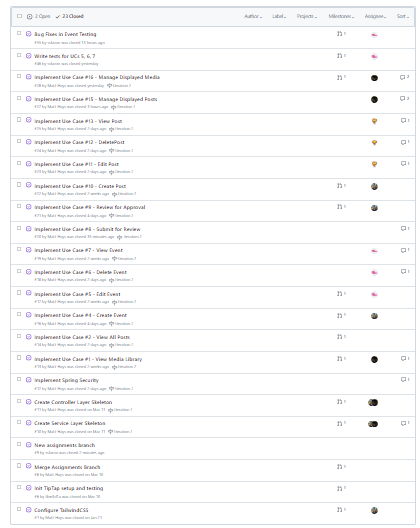
\includegraphics[width=0.8\textwidth]{images/ClosedIssues.png}
    \centering
    \caption{23 Closed Issues in the Incredibles GitHub Repository}
\end{figure}

\begin{figure}[H]
    \centering
    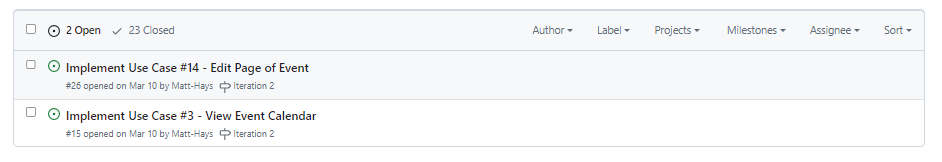
\includegraphics[width=0.8\textwidth]{images/OpenIssues.png}
    \centering
    \caption{2 Remaining Open Issues in the Incredibles GitHub Repository}
\end{figure}

\begin{figure}[H]
    \centering
    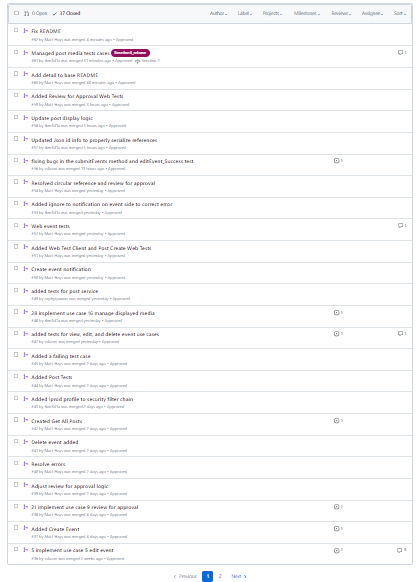
\includegraphics[width=0.8\textwidth]{images/PullRequests1.png}
    \centering
    \caption{37 Closed Pull Requests in the Incredibles GitHub Repository: Page 1}
\end{figure}

\begin{figure}[H]
    \centering
    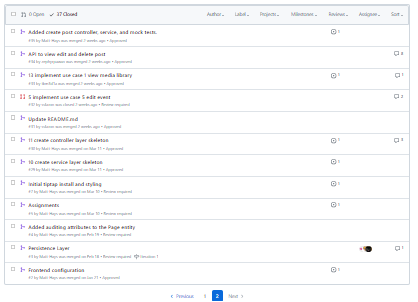
\includegraphics[width=0.8\textwidth]{images/PullRequests2.png}
    \centering
    \caption{37 Closed Pull Requests in the Incredibles GitHub Repository: Page 2}
\end{figure}

\subsubsection{Documentation}

The full Postman collection with 24 API requests is included in the root of the project submission zip. Full API documentation to accompany this Postman collection has been published and is publicly available at \href{https://documenter.getpostman.com/view/25830847/2sA3BheZms}{this link}.

\subsubsection{Test Report}

A full test report is included in the root of the project submission zip. All 26 tests pass with no failures, errors, or skipped tests.